%\documentclass[anonymous, sigconf]{acmart}
\documentclass[sigconf]{acmart}
\settopmatter{printacmref=false}
%%
%% \BibTeX command to typeset BibTeX logo in the docs
\AtBeginDocument{%
  \providecommand\BibTeX{{%
    Bib\TeX}}}

% %% Rights management information.  This information is sent to you
% %% when you complete the rights form.  These commands have SAMPLE
% %% values in them; it is your responsibility as an author to replace
% %% the commands and values with those provided to you when you
% %% complete the rights form.
% \setcopyright{acmlicensed}
% \copyrightyear{2018}
% \acmYear{2018}
\acmDOI{}
%% These commands are for a PROCEEDINGS abstract or paper.
\acmConference[ASP-DAC '27]
{32nd Asia and South Pacific Design Automation Conference}
{January 25--28, 2027}
{Tokyo, Japan}
% %
% %  Uncomment \acmBooktitle if the title of the proceedings is different
% %  from ``Proceedings of ...''!
% %
% %\acmBooktitle{Woodstock '18: ACM Symposium on Neural Gaze Detection,
% %  June 03--05, 2018, Woodstock, NY}
\acmISBN{}

\usepackage{doi}
%%
%% Submission ID.
%% Use this when submitting an article to a sponsored event. You'll
%% receive a unique submission ID from the organizers
%% of the event, and this ID should be used as the parameter to this command.
%%\acmSubmissionID{123-A56-BU3}

%%
%% For managing citations, it is recommended to use bibliography
%% files in BibTeX format.
%%
%% You can then either use BibTeX with the ACM-Reference-Format style,
%% or BibLaTeX with the acmnumeric or acmauthoryear sytles, that include
%% support for advanced citation of software artefact from the
%% biblatex-software package, also separately available on CTAN.
%%
%% Look at the sample-*-biblatex.tex files for templates showcasing
%% the biblatex styles.
%%
%%
%% The majority of ACM publications use numbered citations and
%% references.  The command \citestyle{authoryear} switches to the
%% "author year" style.
%%
%% If you are preparing content for an event
%% sponsored by ACM SIGGRAPH, you must use the "author year" style of
%% citations and references.
%% Uncommenting
%% the next command will enable that style.
%%\citestyle{acmauthoryear}


%%
%% end of the preamble, start of the body of the document source.
\begin{document}

%%
%% The "title" command has an optional parameter,
%% allowing the author to define a "short title" to be used in page headers.
\title{ZhuLong: Execution-Grounded LLM Agent for EDA Scripting with Offline API Self-Exploration}

%%
%% The "author" command and its associated commands are used to define
%% the authors and their affiliations.
%% Of note is the shared affiliation of the first two authors, and the
%% "authornote" and "authornotemark" commands
%% used to denote shared contribution to the research.
% ============ 作者部分 ============
% 使用 tabular 实现紧凑排版（注：PDF 元数据会丢失）
\author{%
  \begin{tabular}{c}
    Yang Liu \quad Shiwei Hou \quad Xiyuan Chen \quad Yu Wang \quad Sen Yuan \\[1pt]
    {\small \{paul.liu, shiwei.hou\}@cxmt.com \quad chenxiyuan@mail.ustc.edu.cn} \\[4pt]
    Qirui Gan \quad Shao You \quad Feifan Chen \quad Wencheng Li \quad Shuyang Hu \\[1pt]
    Yongzhou Liu \quad Emma Xia \quad Xiaojing Lu \quad Hao Wang \quad Fan Xu \quad Yanfeng Li
  \end{tabular}
}

\affiliation{%
  \institution{Changxin Memory Technologies, Inc.}
  \country{China}
}

\renewcommand{\shortauthors}{Liu et al.}

%%
%% The abstract is a short summary of the work to be presented in the
%% article.
\begin{abstract}
    EDA scripting with tool-specific, often undocumented APIs remains a long-tail 
    bottleneck that existing LLMs fail to address. This paper presents 
    \textbf{ZhuLong}, an execution-grounded LLM coding agent for PyAether and 
    SKILL that combines API retrieval, documentation inspection, and sandbox 
    execution via unified MCP tools, augmented by an offline \textbf{API 
    self-exploration mechanism} that infers undocumented API behaviors through 
    counterfactual experimentation.
    % 使用工具特定且常无文档的EDA API进行脚本编写，仍是现有LLM无法解决的
    % 长尾瓶颈。本文提出\textbf{ZhuLong}，一个面向PyAether和SKILL的执行驱动
    % LLM代码智能体，通过统一的MCP工具组合API检索、文档查阅和沙盒执行，
    % 并辅以离线\textbf{API自探索机制}，通过反事实实验推断未文档化的API行为。
    
    We evaluate ZhuLong on \textbf{EDA-Eval-PyAether}, a benchmark of 158
    real-world tasks with assertion-based execution, where the complete system
    achieves \textbf{78.5\%} Pass@1 in the commercial Empyrean Aether
    environment, substantially outperforming a pure LLM baseline (\textbf{23.6\%}). Ablation studies identify sandbox execution as the dominant
    performance driver (41.2 pp drop when removed), with the self-exploration
    mechanism contributing an additional 3.2 pp accuracy gain and a 22.1\%
    reduction in per-task tool calls. On 20 interactive tasks involving unsaved
    layouts and schematics, ZhuLong achieves 60.0\% Pass@1 for PyAether and
    50.0\% for SKILL. 
    % 我们在\textbf{EDA-Eval-PyAether}上评估ZhuLong，该基准包含158个真实任务，
    % 采用基于断言的执行验证，完整系统在商业Empyrean Aether环境中达到
    % \textbf{78.5\%}的Pass@1，显著优于纯LLM基线（\textbf{23.6\%}）。消融实验表明，沙盒执行是性能提升的主导因素
    % （移除后下降41.2个百分点），自探索机制在贡献额外3.2个百分点准确率提升的
    % 同时，将每任务工具调用次数减少22.1\%。在20个涉及未保存版图和原理图的
    % 交互任务中，ZhuLong在PyAether上达到60.0\% Pass@1，在SKILL上达到
    % 50.0\% Pass@1。
\end{abstract}

\keywords{LLM Agents for EDA, EDA Scripting, Code Generation, Sandbox Execution, API Self-Exploration}

\begin{CCSXML}
<ccs2012>
   <concept>
       <concept_id>10010583.10010682.10010712.10010715</concept_id>
       <concept_desc>Hardware~Software tools for EDA</concept_desc>
       <concept_significance>500</concept_significance>
       </concept>
 </ccs2012>
\end{CCSXML}

\ccsdesc[500]{Hardware~Software tools for EDA}

% %%
% %% The code below is generated by the tool at http://dl.acm.org/ccs.cfm.
% %% Please copy and paste the code instead of the example below.
% %%
% \begin{CCSXML}
% <ccs2012>
%  <concept>
%   <concept_id>00000000.0000000.0000000</concept_id>
%   <concept_desc>Do Not Use This Code, Generate the Correct Terms for Your Paper</concept_desc>
%   <concept_significance>500</concept_significance>
%  </concept>
%  <concept>
%   <concept_id>00000000.00000000.00000000</concept_id>
%   <concept_desc>Do Not Use This Code, Generate the Correct Terms for Your Paper</concept_desc>
%   <concept_significance>300</concept_significance>
%  </concept>
%  <concept>
%   <concept_id>00000000.00000000.00000000</concept_id>
%   <concept_desc>Do Not Use This Code, Generate the Correct Terms for Your Paper</concept_desc>
%   <concept_significance>100</concept_significance>
%  </concept>
%  <concept>
%   <concept_id>00000000.00000000.00000000</concept_id>
%   <concept_desc>Do Not Use This Code, Generate the Correct Terms for Your Paper</concept_desc>
%   <concept_significance>100</concept_significance>
%  </concept>
% </ccs2012>
% \end{CCSXML}

% \ccsdesc[500]{Do Not Use This Code~Generate the Correct Terms for Your Paper}
% \ccsdesc[300]{Do Not Use This Code~Generate the Correct Terms for Your Paper}
% \ccsdesc{Do Not Use This Code~Generate the Correct Terms for Your Paper}
% \ccsdesc[100]{Do Not Use This Code~Generate the Correct Terms for Your Paper}

% \received{20 February 2007}
% \received[revised]{12 March 2009}
% \received[accepted]{5 June 2009}

%%
%% This command processes the author and affiliation and title
%% information and builds the first part of the formatted document.
\maketitle


\section{Introduction}
\label{sec:introduction}

Large language models (LLMs) have demonstrated strong capabilities in general-purpose code generation \cite{vaswani2017attention, openai2023gpt4, yang2025qwen3}. However, applying LLMs to EDA scripting—where engineers routinely manipulate in-memory design databases, create layout instances, route schematics, and query netlists—remains challenging. First, EDA APIs are long-tailed and tool-specific; many rarely appear in public training corpora. Second, correctness cannot be verified statically: it depends on observable side effects in a real EDA environment, such as modified layouts or updated schematics. Third, without execution feedback, static generation cannot diagnose errors or iteratively refine incorrect code \cite{chen2024dawning, blocklove2024eda}. Existing LLM-based EDA work has mainly focused on HDL generation \cite{thakur2023verigen, liu2023rtlcoder}, while scripting with real tool APIs—especially with incomplete documentation and sandbox execution—remains underexplored.
% 大语言模型在通用代码生成方面表现强大，但应用于EDA脚本——工程师日常操作内存中的设计数据库、创建版图实例、布线原理图、查询网表——仍面临挑战。第一，EDA API具有长尾性和工具特定性，许多很少出现在公开训练语料中。第二，正确性无法静态验证：它取决于真实EDA环境中的可观察副作用，如版图修改或原理图更新。第三，没有执行反馈，静态生成无法诊断错误或迭代修正代码。现有LLM-for-EDA工作主要集中在HDL生成，而面向真实工具API、沙盒执行和不完整文档的脚本生成仍研究不足。

This paper presents \textbf{ZhuLong}, an execution-grounded LLM coding agent for PyAether and SKILL. Named after a mythical creature whose opened eyes bring light, ZhuLong aims to illuminate opaque EDA APIs and automate tool-specific scripting workflows. Built on Cline-CLI \cite{cline2024cline}, ZhuLong extends three MCP tools \cite{lee2025autoeda}—\texttt{search\_apis}, \texttt{get\_api\_details}, and \texttt{run\_code}—that form a closed loop: retrieve candidate APIs, inspect their documentation, execute code in the EDA environment with execution feedback, and iteratively refine based on observed errors or outputs. All tools accept a unified \texttt{lang} parameter, supporting both PyAether and SKILL with identical agent logic. To further address incomplete or outdated documentation, ZhuLong introduces an offline \textbf{API self-exploration mechanism} that proactively explores undocumented API behaviors in the sandbox via \textbf{counterfactual experimentation}—deliberately testing alternative parameter values, observing execution outcomes, inferring constraints and usage patterns, and storing the discovered information as enhanced API documentation for future queries.
% 本文提出\textbf{ZhuLong}，一个面向PyAether和SKILL的执行驱动LLM代码智能体。其名源自中国神话中睁眼带来光明的神兽，寓意照亮不透明的EDA API并自动化工具特定的脚本流程。ZhuLong基于Cline-CLI构建，扩展三个MCP工具——\texttt{search\_apis}、\texttt{get\_api\_details}和\texttt{run\_code}——形成闭环：检索候选API、查阅文档、在沙盒EDA环境中执行代码、基于观察到的错误或输出迭代修正。所有工具接受统一的\texttt{lang}参数，以相同智能体逻辑同时支持PyAether和SKILL。为了进一步解决文档不完整或过时的问题，ZhuLong引入了离线\textbf{API自探索机制}，通过沙盒中的\textbf{反事实实验}主动探索未文档化的API行为——有意识地测试不同参数取值、观察执行结果、推断约束和使用模式、将发现的信息存储为增强的API文档供后续查询使用。

The main contributions are:
\begin{itemize}
    \item \textbf{First execution-grounded agent for commercial EDA scripting.} We present the first system that validates execution feedback in PyAether and SKILL via sandbox execution, delivering a +43 pp accuracy gain over static RAG.
    % 首个面向商业EDA脚本的执行驱动智能体。我们提出了首个通过沙盒执行验证PyAether和SKILL执行反馈的系统，相比静态RAG带来+43个百分点的准确率提升。
    \item \textbf{Offline API self-exploration for EDA.} A complementary mechanism that contributes +3.2 pp accuracy gain and reduces the average number of tool calls per trace by 22.1\% through counterfactual experimentation on undocumented APIs. To our knowledge, this is the first mechanism that proactively discovers and codifies undocumented API behaviors in the EDA domain.
    % \textbf{面向EDA的离线API自探索。}一种互补机制，通过对未文档化API进行反事实实验，贡献了+3.2个百分点的准确率提升，并将每条trace的平均工具调用次数减少22.1\%。据我们所知，这是首个在EDA领域中主动发现并系统记录未文档化API行为的机制。
    \item \textbf{EDA-Eval-PyAether: the first public benchmark for PyAether scripting.} A benchmark of 158 real-world tasks with assertion-based execution, enabling rigorous evaluation of LLM-generated EDA scripts. The complete ZhuLong system achieves 78.5\% Pass@1 on this benchmark.
    % EDA-Eval-PyAether：首个PyAether脚本公开评测集。包含158个真实任务的基准，采用基于断言的执行验证，支持对LLM生成的EDA脚本进行严格评估。完整ZhuLong系统在该基准上达到78.5\%的Pass@1。
\end{itemize}
\section{Background and Motivation}
\label{sec:background}

We target two widely-used EDA scripting interfaces: PyAether for Empyrean Aether \cite{empyrean_pyaether} and SKILL for Cadence Virtuoso \cite{cadence2024virtuoso}. Despite their prevalence, scripting for both environments poses challenges beyond what generic LLM code generators can address, and the community lacks basic infrastructure to measure progress.
% 我们关注两个广泛使用的EDA脚本接口：面向Empyrean Aether的PyAether和面向Cadence Virtuoso的SKILL。尽管它们被广泛使用，但这两个环境的脚本编写面临着通用LLM代码生成器无法解决的挑战，而且整个社区甚至缺乏衡量进展的基本基础设施。

\textbf{EDA scripting is fundamentally different.} Prior work on LLM code generation has succeeded in domains where correctness is verified by unit tests \cite{chen2021evaluating, austin2021program}. EDA scripting presents three distinct challenges: (i) APIs are long-tailed, tool-specific, and poorly documented; (ii) correctness depends on side effects in a live, stateful database, not return values; and (iii) no benchmark exists to evaluate whether generated scripts actually work.
% \textbf{EDA脚本根本不同。} 此前LLM代码生成的工作在可通过单元测试验证的领域取得了成功。EDA脚本编写面临三个不同挑战：(i) API长尾、工具特定、文档不完整；(ii) 正确性取决于实时有状态数据库的副作用，而非返回值；(iii) 不存在评测集来验证生成的脚本是否真正有效。

\textbf{Prior work stops short of execution.} Recent efforts like LayoutCopilot \cite{liu2025layoutcopilot}, ChaTCL \cite{rui2025chatcl}, and RAG-EDA \cite{pu2024rag} combine LLMs with static knowledge bases. Yet they all share a critical limitation: they do not execute generated code. Correctness is assessed by human judgment \cite{liu2025layoutcopilot, rui2025chatcl} or retrieval quality \cite{pu2024rag}, not by whether the script actually modifies a layout. Consequently, errors go undiagnosed, and the gap between "looks plausible" and "actually works" remains unbridged.
% \textbf{已有工作止步于执行。} LayoutCopilot、ChaTCL和RAG-EDA将LLM与静态知识库结合，但都存在关键局限：不执行生成的代码。正确性通过人工判断或检索质量评估，而非观察脚本是否真正修改了版图。因此错误无法诊断，"看起来对"与"真正能用"之间的鸿沟始终未能弥合。

\textbf{The root problem: no benchmark, no progress.} Without a standardized benchmark, the community cannot systematically compare approaches or measure progress—each prior work uses ad-hoc tasks with different protocols. Recent concurrent benchmarks for Tcl/Innovus flows \cite{xu2026iscript, li2026pdagent} confirm the growing recognition of this gap, yet target different toolchains. A dedicated PyAether/SKILL benchmark remains absent.
% \textbf{根本问题：没有评测集，就没有进展。} 没有标准化的评测集，社区无法系统比较不同方法或衡量进展——每个已有工作使用不同的任务和协议。近期针对Tcl/Innovus流程的同期评测集表明这一空白正被广泛认识，但它们针对的是不同工具链。PyAether/SKILL领域仍然缺乏专用评测基准。

\textbf{Our approach.} ZhuLong addresses the technical challenges through sandbox execution feedback—closing the loop from generation to execution to refinement—complemented by an offline \textbf{API self-exploration mechanism}. Crucially, we introduce \textbf{EDA-Eval-PyAether}, the first standardized benchmark for PyAether scripting. Together, these contributions establish both the methodology and the measurement infrastructure for advancing LLM-based EDA scripting.
% \textbf{我们的方法。} ZhuLong通过沙盒执行反馈应对技术挑战——闭环从生成到执行到修正——辅以离线API自探索机制。更重要的是，我们引入EDA-Eval-PyAether，首个面向PyAether脚本的标准化评测集。三者共同构成了推进LLM-driven EDA脚本编写的方法论和测量基础设施。
\section{System Design}
\label{sec:system}

\subsection{Overall Architecture}
\label{sec:overall-architecture}

ZhuLong is built on Cline-CLI \cite{cline2024cline}, an open-source framework for autonomous coding agents, extended with EDA-specific retrieval, documentation, and execution capabilities. We choose Cline-CLI for its mature permission controls, human-in-the-loop support, and enterprise readiness. As shown in Figure~\ref{fig:architecture}, the system comprises three components: the LLM-based agent runtime, the API knowledge base, and the EDA execution environment. The agent interacts with these components through three MCP tools, while an offline \textbf{API self-exploration mechanism} pre-augments the API knowledge base before runtime.
% ZhuLong基于Cline-CLI \cite{cline2024cline}构建，这是一个开源自主代码智能体框架，我们扩展了EDA特定的检索、文档查阅和执行能力。选择Cline-CLI是因为其成熟的权限控制、人在闭环支持和企业级就绪能力。如图~\ref{fig:architecture}所示，系统包括三个组件：基于LLM的智能体运行时、API知识库和EDA执行环境。智能体通过三个MCP工具与这些组件交互，离线\textbf{API自探索机制}在运行前预增强API知识库。

\begin{figure*}[t]
\centering
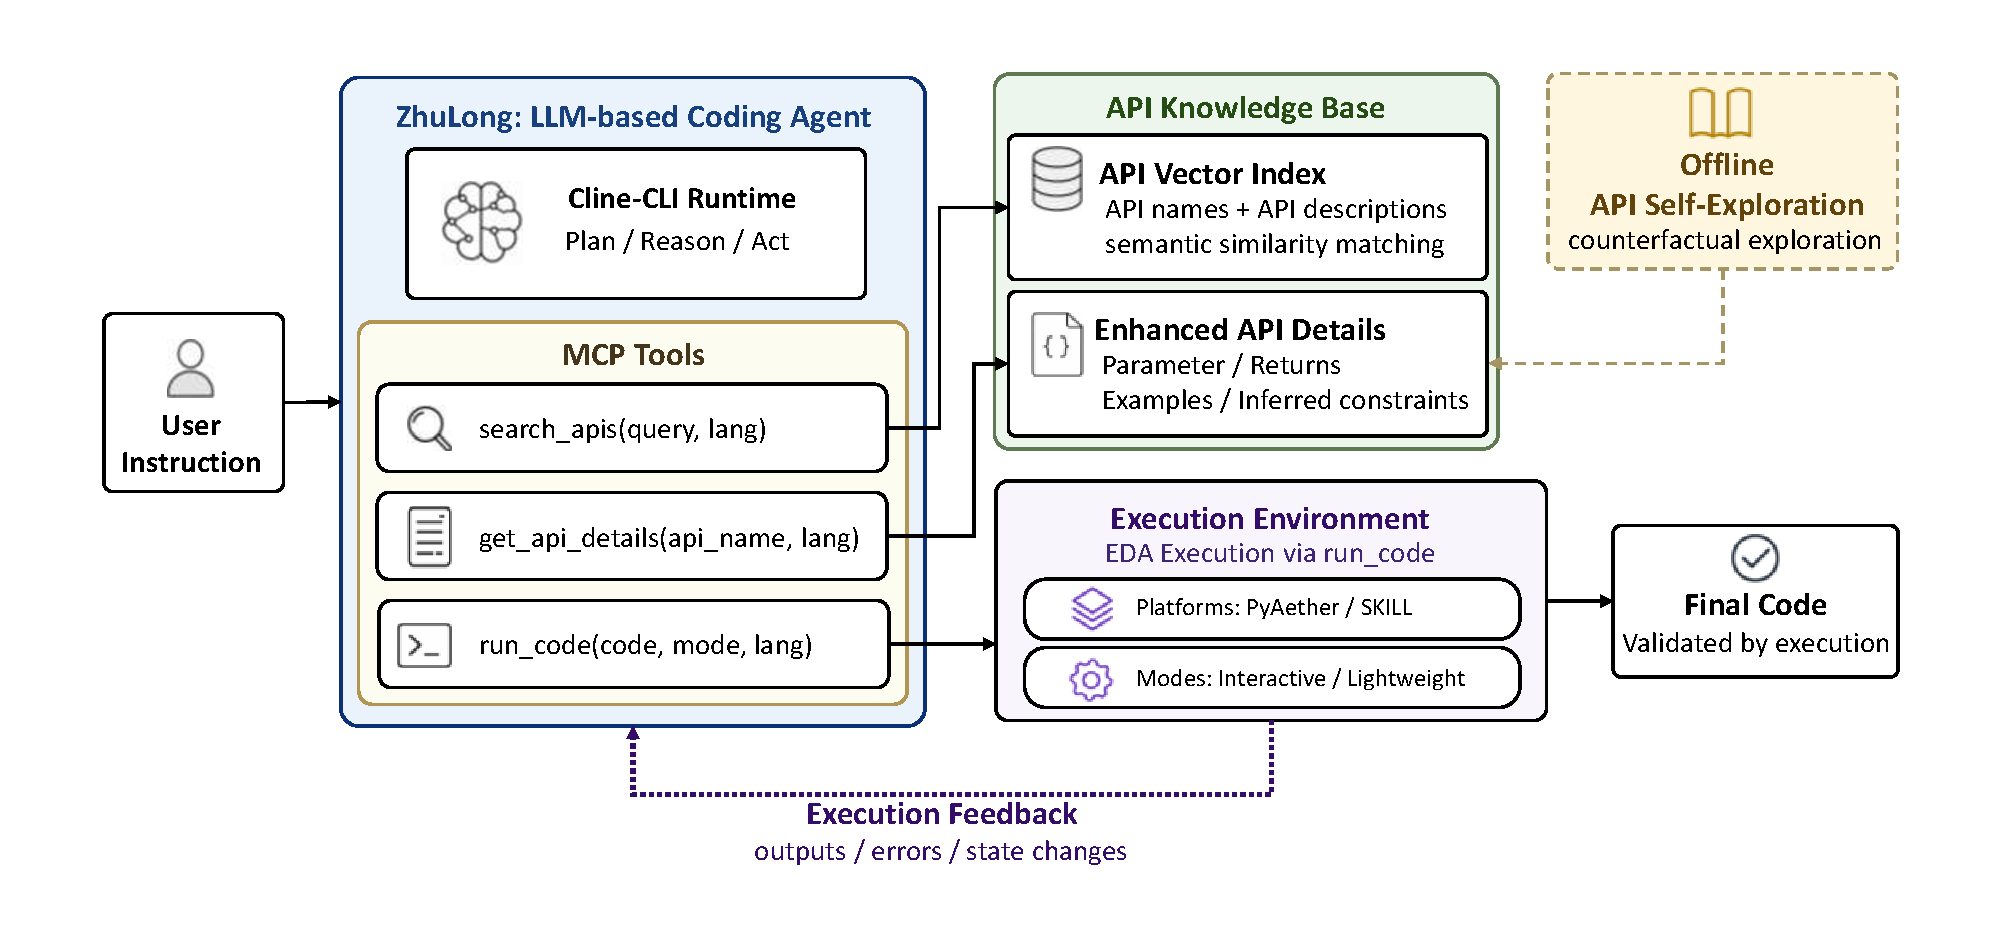
\includegraphics[width=0.9\textwidth]{figures/zhulong_arch_2.pdf}
\caption{ZhuLong system architecture. The agent interacts with API retrieval, enhanced documentation, and EDA execution via three unified MCP tools. Offline self-exploration augments the knowledge base before runtime, and execution feedback supports iterative refinement.}
% ZhuLong系统架构。智能体通过三个统一的MCP工具与API检索、增强文档和EDA执行环境交互。离线自探索在运行前增强知识库，执行反馈支持迭代优化。
\label{fig:architecture}
\end{figure*}

\subsection{Three MCP Tools}
\label{sec:mcp-tools}

ZhuLong extends three MCP tools \cite{mcp2024protocol}, each accepting a unified \texttt{lang} parameter (\texttt{pyaether} or \texttt{skill}) to support both platforms with identical agent logic:
% ZhuLong扩展了三个MCP工具 \cite{mcp2024protocol}，每个工具接受统一的\texttt{lang}参数（\texttt{pyaether}或\texttt{skill}），以相同智能体逻辑支持两个平台：

\begin{itemize}
    \item \texttt{search\_apis(query, lang)} retrieves relevant APIs via semantic and keyword-based search. We index APIs by name and description using BGE-M3 embeddings \cite{bge2024} with FAISS \cite{douze2024faiss} for efficient similarity search, returning the top-$K$ results ($K=5$ by default) with confidence scores and descriptions.
    % \texttt{search\_apis(query, lang)}通过语义和关键词检索相关API。我们使用BGE-M3嵌入 \cite{bge2024}对API名称和描述建索引，FAISS \cite{faiss2017}支持高效相似度搜索，返回top-$K$结果（默认$K=5$），附带置信度分数和描述。
    
    \item \texttt{get\_api\_details(api\_name, lang)} fetches comprehensive documentation for a specified API, including parameter types, return values, and examples. The returned documentation is augmented by the offline API self-exploration mechanism (Section~\ref{sec:selfdoc}) when available, enriching incomplete specifications with constraints and usage patterns discovered via sandbox exploration.
    % \texttt{get\_api\_details(api\_name, lang)}获取指定API的完整文档，包括参数类型、返回值和示例。当可用时，返回的文档由离线API自探索机制（第~\ref{sec:selfdoc}节）增强，补充通过沙盒探索发现的约束和使用模式。
    
    \item \texttt{run\_code(code, mode, lang)} executes the generated code in the EDA environment. It supports two modes: (1) \textbf{lightweight}—runs in a sandboxed environment without a GUI session (standalone PythonE for PyAether, or SKILL in batch mode for Virtuoso), capturing outputs, errors, and state changes for iterative refinement; (2) \textbf{interactive}—runs inside an open EDA session via the agent-EDA bridge (socket communication), enabling operations on unsaved layouts and schematics.
    % \texttt{run\_code(code, mode, lang)}在EDA环境中执行生成的代码。支持两种模式：（1）\textbf{轻量模式}——在沙盒化环境中运行，无需GUI会话（PyAether使用独立PythonE环境，Virtuoso使用SKILL批处理模式），捕获输出、错误和状态变化供迭代优化使用；（2）\textbf{交互模式}——通过agent-EDA桥接（socket通信）在已打开的EDA会话内运行，支持操作未保存的版图和原理图。
\end{itemize}

\subsection{Agent Workflow}
\label{sec:agent-workflow}

The agent iteratively refines its output through execution feedback \cite{cline2024cline}. A typical trajectory begins with reasoning over the user instruction, followed by API retrieval via \texttt{search\_apis} when needed. Candidate APIs are then inspected via \texttt{get\_api\_details}, and code is generated accordingly. The agent executes the code via \texttt{run\_code}, observes the result, and re-plans—revising the code, retrieving alternative APIs, or terminating. This loop continues until success or the agent determines further attempts are unlikely to succeed. The agent is not constrained to a fixed sequence; it may skip retrieval when it already knows the required API, or conduct multiple rounds of retrieval when initial results lack confidence.
% 智能体通过执行反馈迭代优化其输出 \cite{cline2024cline}。典型轨迹始于对用户指令的推理，需要时通过\texttt{search\_apis}检索API，然后通过\texttt{get\_api\_details}查阅候选API的文档，据此生成代码。智能体通过\texttt{run\_code}执行代码、观察结果并重规划——修改代码、检索替代API或终止。此循环持续至成功或智能体判断继续尝试不太可能成功。智能体不受固定序列约束——已知所需API时可跳过检索，初始结果置信度不足时可进行多轮检索。
\section{Offline API Self-Exploration Mechanism}
\label{sec:selfdoc}

API documentation in EDA tools is often incomplete, omitting parameter constraints, return structures, and error conditions. Prior work addresses documentation gaps through retrieval-based augmentation \cite{pu2024rag} or static knowledge graphs \cite{liu2025layoutcopilot}—both of which rely on what is already documented. When documentation is absent, these approaches provide no remedy.

% EDA工具的API文档往往不完整，省略了参数约束、返回值结构和错误条件。已有工作通过检索增强或静态知识图谱来弥补文档不足——但两者都依赖于已有文档的内容。当文档完全缺失时，这些方法无法提供任何补救。

ZhuLong takes a different approach: instead of waiting for documentation to exist, it \textbf{proactively discovers} API behaviors through offline counterfactual experimentation in the sandbox. For each target API, the self-exploration agent reads whatever documentation is available, identifies gaps—e.g., unspecified parameter ranges, undocumented return fields, or ambiguous error semantics—and generates targeted test scripts to probe them. It executes these scripts via \texttt{run\_code}, observes outcomes, and iteratively refines its hypotheses about what the API accepts and returns. The exploration agent autonomously decides what to test next and when to stop, based on its current confidence.

% ZhuLong采取不同的策略：不等文档存在，而是通过沙盒中的离线反事实实验\textbf{主动发现} API行为。对于每个目标API，自探索智能体阅读现有文档，识别其中的空白——如未指定的参数范围、未文档化的返回字段或模糊的错误语义——并生成针对性的测试脚本进行探测。它通过\texttt{run\_code}执行这些脚本，观察结果，并迭代修正关于API接受什么参数、返回什么数据的假设。探索智能体根据当前置信度自主决定下一步测试什么以及何时停止。

Concretely, the exploration agent constructs counterfactual hypotheses—e.g., whether a parameter accepts an empty list, whether a numeric argument allows negative values, or whether a return value contains a specific field—and designs minimal test cases to validate each. Execution outcomes (success, error, exception, or unexpected return structure) reveal actual constraints. Over multiple rounds, the agent builds a behavioral model of each API, capturing parameter constraints, return structures, error conditions, and side effects.

% 具体而言，探索智能体构造反事实假设——例如参数是否接受空列表、数值参数是否允许负值、返回值是否包含特定字段——并设计最小测试用例验证每个假设。执行结果（成功、错误、异常或意外的返回结构）揭示实际约束。经过多轮迭代，智能体构建了每个API的行为模型，捕获参数约束、返回值结构、错误条件和副作用。

This offline process runs once per API; the enriched documentation is stored in the API knowledge base and served at runtime via \texttt{get\_api\_details}, incurring no runtime overhead. The resulting documentation is more complete than what is available in official sources, and directly reflects the API's actual behavior rather than its intended or assumed behavior.

% 该离线过程每个API运行一次；增强后的文档存储在API知识库中，运行时通过\texttt{get\_api\_details}提供，不产生运行时开销。生成的文档比官方来源更完整，直接反映API的实际行为而非预期或假定的行为。
\section{Benchmark Construction}
\label{sec:benchmark}

\subsection{Dataset: EDA-Eval-PyAether}

To evaluate LLM-based code generation for PyAether, we constructed \textbf{EDA-Eval-PyAether}, a benchmark of 158 tasks. Tasks were collected from four sources: API references (61.4\%), documentation examples (27.2\%), internal training materials (7.6\%), and anonymized CAD practical cases (3.8\%). Each task underwent manual review by EDA domain experts.
% 为了评估基于LLM的PyAether代码生成，我们构建了\textbf{EDA-Eval-PyAether}评测集，包含158个任务。任务收集自四个来源：API参考文档（61.4\%）、官方文档示例（27.2\%）、内部培训材料（7.6\%）和脱敏的CAD实际案例（3.8\%）。每个任务均由EDA领域专家进行了人工审核。

Table~\ref{tab:scenario-distribution} shows the distribution of tasks across different EDA scenarios. Layout and Schematic operations constitute the majority (70.2\%), reflecting the core focus of PyAether usage in physical design workflows.
% 表~\ref{tab:scenario-distribution}展示了任务在不同EDA场景中的分布。Layout和Schematic操作占大多数（70.2\%），反映了PyAether在物理设计工作流中的核心使用场景。

\begin{table}[htbp]
\centering
\caption{Task distribution by scenario}
\label{tab:scenario-distribution}
\begin{tabular}{lcc}
\toprule
\textbf{Scenario} & \textbf{Tasks} & \textbf{Percentage} \\
\midrule
Layout & 64 & 40.5\% \\
Schematic & 47 & 29.7\% \\
Design Management & 24 & 15.2\% \\
Others & 23 & 14.6\% \\
\midrule
Total & 158 & 100\% \\
\bottomrule
\end{tabular}
\end{table}
% 表：按场景划分的任务分布。

\subsection{Evaluation Protocol}

Each task consists of a natural language prompt, a function signature, and assertion-based test code. A task is considered passed if the generated code executes in the PyAether sandbox without errors and all assertions pass. The primary metric is Pass@1 \cite{chen2021evaluating}:
% 每个任务包含三个部分：自然语言提示、函数签名、以及基于断言的测试代码。如果生成的代码在PyAether沙盒中无错误执行且所有断言通过，则该任务被视为通过。主要指标为Pass@1 \cite{chen2021evaluating}：

\[
\text{Pass@1} = \frac{\text{\# tasks with all assertions passed}}{\text{Total tasks}} \times 100\%
\]
% \[
% \text{Pass@1} = \frac{\text{所有断言均通过的任务数}}{\text{总任务数}} \times 100\%
% \]
\section{Experiments}
\label{sec:experiments}

\subsection{Experimental Setup}
\label{sec:exp-setup}

\subsubsection{Research Questions}

This evaluation aims to answer four research questions: (RQ1) whether sandbox execution improves code generation accuracy over static generation; (RQ2) whether the self-exploration mechanism provides measurable benefits beyond sandbox execution alone, in terms of both accuracy and efficiency; (RQ3) whether vector-based retrieval outperforms grep-based keyword search for API discovery; and (RQ4) how different index construction strategies affect retrieval effectiveness.
% 本评估旨在回答四个研究问题：(RQ1) 沙盒执行相比静态生成是否提升了代码生成准确率；(RQ2) 自探索机制在沙盒执行之外是否带来了可测量的准确率和效率增益；(RQ3) 向量检索在API发现上是否优于grep关键词搜索；(RQ4) 不同的索引构建策略如何影响检索效果。

\subsubsection{Benchmark and Evaluation Protocol}

We evaluate ZhuLong on \textbf{EDA-Eval-PyAether}, a benchmark of 158 real-world PyAether scripting tasks. Following the evaluation protocol defined in Section~\ref{sec:benchmark}, we adopt \textbf{Pass@1} (execution success rate) as the primary metric. During evaluation, the agent is allowed up to \textbf{2 re-planning rounds} per task (i.e., up to three complete runs), following the self-correction loop described in Section~\ref{sec:agent-workflow}; timeout is set to 2500 seconds per execution.
% 评测集与评估协议。我们在\textbf{EDA-Eval-PyAether}上评估ZhuLong，该评测集包含158个真实PyAether脚本任务。遵循第\ref{sec:benchmark}节定义的评估协议，我们采用\textbf{Pass@1}（执行成功率）作为主要指标。评估过程中，智能体在每个任务上允许最多\textbf{2轮重新规划}（即最多进行3次完整运行），遵循第\ref{sec:agent-workflow}节描述的自校正循环；每次执行超时时间设为2500秒。

\subsubsection{Baselines and ZhuLong Variants}

To isolate the contribution of each component, we establish two baselines and three ZhuLong variants, as shown in Table~\ref{tab:configurations}. ZhuLong variants default to vector retrieval using a name+description index.
% 基线与ZhuLong变体。为了隔离每个组件的贡献，我们建立了两个基线和三个ZhuLong变体，如表~\ref{tab:configurations}所示。ZhuLong变体默认使用名称+描述索引进行向量检索。

\begin{table}[htbp]
\centering
\caption{Configurations and their components}
\label{tab:configurations}
\begin{tabular}{lccc}
\toprule
\textbf{Configuration} & \textbf{Retrieval} & \textbf{Sandbox} & \textbf{Self-Expl.} \\
\midrule
Baseline 1 (Pure LLM) & \ding{55} & \ding{55} & \ding{55} \\
Baseline 2 (RAG) & \ding{51} & \ding{55} & \ding{55} \\
ZhuLong w/o Self-Expl. & \ding{51} & \ding{51} & \ding{55} \\
ZhuLong w/o Sandbox & \ding{51} & \ding{55} & \ding{51} \\
ZhuLong w/o Retrieval & \ding{55} & \ding{51} & \ding{51} \\
\textbf{ZhuLong} (Full) & \ding{51} & \ding{51} & \ding{51} \\
\bottomrule
\end{tabular}
\end{table}
% 表：配置及其组件。ZhuLong（完整）为完整系统，其余为消融变体。
% Self-Expl. = Self-Exploration mechanism.

\subsubsection{LLM Backbones}

All main experiments use DeepSeek-V4-Flash as the primary backbone. To understand the impact of different LLMs, we additionally evaluate DeepSeek-V3.2, GLM-5.1, DeepSeek-V4-Pro, Kimi-K2.6, and Doubao-Seed-2.0-Pro.
% LLM主干。所有主要实验使用DeepSeek-V4-flash作为主要主干。为了解不同LLM的影响，我们还评估了DeepSeek-V3.2、GLM-5.1、DeepSeek-V4-Pro、Kimi-K2.6和Doubao-Seed-2.0-Pro。

\subsection{Main Results and Ablation}
\label{sec:exp-results}

We further ablate the number of re-planning rounds $n \in \{0, 1, 2\}$.
% 我们进一步消融重新规划轮数$n \in \{0, 1, 2\}$。

Table~\ref{tab:main-ablation} presents the progressive build-up (top), the
iteration budget ablation (middle), and the component ablation (bottom).
The top and bottom blocks use the same re-planning budget of 2 rounds but
present the results from complementary perspectives: the top block shows
the sequential gains from incrementally adding components, with each row
compared against the previous one, whereas the bottom block shows the
performance degradation caused by removing individual components from the
full system. The middle block isolates the effect of the re-planning budget
by comparing 0, 1, and 2 rounds within the full system.
% 表~\ref{tab:main-ablation}呈现了渐进构建（上）、迭代预算消融（中）
% 和组件消融（下）。上、下两部分均采用2轮重新规划预算，但从互补的
% 角度呈现结果：上部分展示逐步添加组件所带来的连续增益，其中每一行
% 均与前一行比较；下部分则展示从完整系统中分别移除各组件后造成的性能
% 下降。中间部分通过在完整系统中比较0、1、2轮重新规划，单独分析重新
% 规划预算的影响。

\begin{table}[htbp]
\centering
\caption{Ablation study results}
\label{tab:main-ablation}
\begin{tabular}{lcc}
\toprule
\textbf{Configuration} & \textbf{Pass@1 (\%)} & \textbf{$\Delta$} \\
\midrule
\multicolumn{3}{l}{\textit{Progressive build-up (vs. previous row)}} \\
Baseline 1: Pure LLM & 23.6 & — \\
Baseline 2: RAG & 32.3 & +8.7 pp \\
ZhuLong w/o Self-Expl. & 75.3 & +43.0 pp \\
\textbf{ZhuLong} (Full) & \textbf{78.5} & \textbf{+3.2 pp} \\
\midrule
\multicolumn{3}{l}{\textit{Iteration budget ablation (vs. ZhuLong Full)}} \\
0 re-planning rounds (single attempt) & 62.7 & -15.8 pp \\
1 re-planning round & 76.0 & -2.5 pp \\
\midrule
\multicolumn{3}{l}{\textit{Component ablation (vs. ZhuLong Full)}} \\
ZhuLong w/o Self-Expl. & 75.3 & -3.2 pp \\
ZhuLong w/o Sandbox & 37.3 & -41.2 pp \\
ZhuLong w/o Retrieval & 34.2 & -44.3 pp \\
\bottomrule
\end{tabular}
\end{table}
% 表：性能构建、迭代预算消融与组件消融研究。上块为渐进构建，"Gain"表示
% 相对于前一行的增量（均为2轮重新规划）；中块为迭代预算消融，下块为组件消融，
% 中块和下块中的"Drop"均表示相对于ZhuLong完整系统（加粗行）的减量。

\subsubsection{Effect of Iteration Budget}
\label{sec:iteration-budget-effect}
%迭代预算的效果

The middle block of Table~\ref{tab:main-ablation} isolates the iteration budget.
% 表~\ref{tab:main-ablation}的中间块分离了迭代预算的影响。
With 0 re-planning rounds, ZhuLong achieves 62.7\% Pass@1, already far above 
the 32.3\% RAG baseline.
% 0轮重新规划时，ZhuLong达到62.7\%的Pass@1，已远高于32.3\%的RAG基线。
One re-planning round raises accuracy to 76.0\% (+13.3 pp, 84.2\% of the total 
achievable gain within two iterations), while the second round adds only 
2.5 pp (final 78.5\%).
% 一轮重新规划将准确率提升至76.0\%（+13.3个百分点，占两轮内可实现总增益的
% 84.2\%），而第二轮仅增加2.5个百分点（最终78.5\%）。
This diminishing return indicates that most recoverable errors are corrected 
within one round; we retain two rounds as the default to capture the remaining 
marginal improvement without excessive overhead.
% 这种边际收益递减表明大多数可恢复错误在一轮内即可修正；我们保留两轮作为默认设置，
% 以在不过度增加开销的前提下捕获剩余的边际增益。

\subsubsection{Effect of Sandbox Execution (RQ1)}

Sandbox execution is the dominant performance driver. Adding it to the RAG baseline raises Pass@1 from 32.3\% to 75.3\%---a gain of \textbf{43.0 percentage points} that accounts for \textbf{78.3\%} of the total improvement from Pure LLM (23.6\%) to ZhuLong (78.5\%). Conversely, removing sandbox execution from ZhuLong drops Pass@1 to 37.3\%, a decline of \textbf{41.2 percentage points}. These results confirm that execution feedback is indispensable: without it, the agent cannot verify correctness, observe API behavior, or iteratively refine its output.
% 沙盒执行的效果（RQ1）。沙盒执行是性能提升的主导因素。将其加入RAG基线后，Pass@1从32.3\%提升至75.3\%——增益\textbf{43.0个百分点}，占从Pure LLM（23.6\%）到ZhuLong（78.5\%）总提升的\textbf{78.3\%}。相反，从ZhuLong中移除沙盒执行后，Pass@1降至37.3\%，下降了\textbf{41.2个百分点}。这些结果确认了执行反馈不可或缺：没有它，智能体无法验证正确性、观察API行为或迭代优化其输出。

We attribute this to two mechanisms. First, execution provides concrete error messages that guide corrections, transforming one-shot generation into iterative search. Second, the agent can experiment with parameter combinations in the sandbox, compensating for gaps in documentation \cite{kumar2026agentforge, jiang2024seed}.
% 我们将此归因于两种机制。第一，执行提供具体的错误信息引导修正，将一次性生成转化为迭代搜索。第二，智能体可以在沙盒中尝试不同的参数组合，弥补文档中的不足。

\subsubsection{Effect of Self-Exploration (RQ2)}

Removing the self-exploration mechanism (while keeping sandbox execution and retrieval) reduces Pass@1 from ZhuLong's 78.5\% to 75.3\%, a drop of 3.2 percentage points. This confirms that the self-exploration mechanism contributes a measurable accuracy gain beyond sandbox execution.
% API自探索的效果（RQ2）。移除自探索机制（同时保留沙盒执行和检索）使Pass@1从ZhuLong的78.5\%降至75.3\%，下降3.2个百分点。这确认了API自探索机制在沙盒执行之外贡献了可测量的准确率提升。

Beyond accuracy, the self-exploration mechanism also improves efficiency. Table~\ref{tab:selfdoc-efficiency} compares tool usage with and without self-exploration. With self-exploration enabled (i.e., ZhuLong), the agent produces more traces (243 vs. 220) because it persists longer with better documentation, yet total tool calls drop by 13.9\% and average calls per trace decrease by 22.1\%.
% 除了准确率，API自探索还提升了效率。表~\ref{tab:selfdoc-efficiency}比较了启用和未启用API自探索时的工具使用情况。启用API自探索后（即ZhuLong），智能体产生了更多的轨迹（243对220），因为更好的文档使其更持久地尝试，但总工具调用次数下降了13.9\%，每次轨迹的平均调用次数下降了22.1\%。

\begin{table}[htbp]
\centering
\caption{Overall tool usage: with vs. without self-exploration}
\label{tab:selfdoc-efficiency}
\begin{tabular}{lcc}
\toprule
\textbf{Metric} & \textbf{w/o Self-Expl.} & \textbf{ZhuLong (Full)} \\
\midrule
Traces & 220 & 243 (+10.5\%) \\
\#Calls & 6,791 & 5,845 (-13.9\%) \\
Avg/Trace & 30.9 & 24.1 (-22.1\%) \\
\midrule
Change & — & \textbf{-946 (-13.9\%)} \\
\bottomrule
\end{tabular}
\end{table}
% 表：整体工具使用情况：启用与未启用API自探索的对比。

The reduction is most pronounced in \texttt{run\_code} (27.0\%, see Table~\ref{tab:tool-breakdown}), indicating that enriched documentation reduces trial-and-error executions. Calls to \texttt{search\_apis} decrease by 12.2\%, while \texttt{get\_api\_details} increase by 9.0\%---a behavioral shift toward more thorough reading before coding.
% \texttt{run\_code}的降幅最为显著（27.0\%），表明增强后的文档减少了试错执行。\texttt{search\_apis}调用下降12.2\%，而\texttt{get\_api\_details}增加9.0\%——这是一种行为转变，即在编码前更充分地阅读文档。

\begin{table}[htbp]
\centering
\caption{Tool-wise call count breakdown}
\label{tab:tool-breakdown}
\begin{tabular}{lcc}
\toprule
\textbf{Tool} & \textbf{w/o Self-Expl.} & \textbf{ZhuLong (Full)} \\
\midrule
\texttt{search\_apis} & 3,203 & 2,812 (-12.2\%) \\
\texttt{get\_api\_details} & 1,151 & 1,255 (+9.0\%) \\
\texttt{run\_code} & 2,437 & 1,778 (-27.0\%) \\
\bottomrule
\end{tabular}
\end{table}
% 表：各工具调用次数明细。

In the absence of sandbox execution, the self-exploration mechanism alone improves Pass@1 from 32.3\% (RAG) to 37.3\% (ZhuLong w/o Sandbox), a gain of 5.0 percentage points. This confirms that enhanced documentation improves generation accuracy even without iterative refinement. The larger gain in the no-sandbox setting (5.0 pp vs. 3.2 pp in ZhuLong) suggests that sandbox execution partially substitutes for pre-explored documentation.
% 在没有沙盒执行的情况下，仅靠API自探索将Pass@1从32.3\%（RAG）提升至37.3\%（ZhuLong w/o Sandbox），增益5.0个百分点。这确认了增强后的文档即使在没有迭代优化的情况下也能提升生成准确率。无沙盒设置下的更大增益（5.0 pp对比ZhuLong中的3.2 pp）表明沙盒执行在一定程度上替代了预探索文档的需求。

\subsubsection{Retrieval Strategy (RQ3) and Index Construction (RQ4)}

Vector-based semantic retrieval outperforms grep-based keyword search by 12.7 percentage points (78.5\% vs. 65.8\%), confirming that natural language queries for EDA tasks rarely match exact API names. For index construction, the name+description index achieves the best result (78.5\%), outperforming description-only (76.0\%) and name-only (75.3\%), indicating that names enable exact matching while descriptions support semantic generalization. Prompt language (English vs. Chinese) shows no material difference, both achieving 78.5\% Pass@1.
% 检索策略（RQ3）与索引构建（RQ4）。基于向量的语义检索比基于grep的关键词搜索高出12.7个百分点（78.5\%对比65.8\%），确认了EDA任务的自然语言查询很少能精确匹配API名称。在索引构建方面，名称+描述联合索引取得了最佳结果（78.5\%），优于仅描述索引（76.0\%）和仅名称索引（75.3\%），表明名称支持精确匹配，而描述支持语义泛化。提示语言（英文 vs. 中文）没有实质性差异，两者均达到78.5\%的Pass@1。

\subsubsection{Impact of LLM Backbone}

Table~\ref{tab:llm-comparison} presents the Pass@1 results for six LLM backbones integrated into the full ZhuLong system. We adopt DeepSeek‑V4‑Flash as the primary backbone across all experiments in this paper, based on a practical trade‑off between model capability and inference cost: its performance is sufficiently strong to support the key findings from both our main experiments and ablation studies, while its cost remains manageable for running the complete set of configurations reported in this work. Kimi‑K2.6 achieves the highest accuracy (83.5\%), outperforming DeepSeek‑V4‑Flash (78.5\%) by 5.0 percentage points. DeepSeek‑V4‑Pro also surpasses this baseline, reaching 81.0\% (+2.5 pp), while GLM‑5.1 ties with DeepSeek‑V4‑Flash at 78.5\%. In contrast, DeepSeek‑V3.2 and Doubao‑Seed‑2.0‑Pro lag notably behind, yielding 67.1\% and 55.7\%, respectively. The spread of 27.8 percentage points between the best and worst performers indicates that the underlying model remains a decisive factor, even with retrieval, sandbox, and self‑exploration in place. Notably, the ranking on this benchmark does not strictly follow the general coding proficiency reported in public leaderboards. This discrepancy suggests that EDA scripting—with its long‑tail APIs and state‑sensitive logic—imposes a distinct set of demands that generic code benchmarks do not adequately capture.
%表~\ref{tab:llm-comparison} 给出了六个LLM主干在完整ZhuLong系统上的Pass@1结果。我们选择DeepSeek‑V4‑flash作为本文所有实验的主干模型，主要基于模型能力与推理成本之间的实际均衡考量：其性能足以支撑主实验和消融实验的核心结论，同时计算开销也在可控范围内，便于完整运行本文报告的全部实验配置。Kimi‑K2.6表现最佳（83.5%），较DeepSeek‑V4‑flash（78.5%）高出5.0个百分点。DeepSeek‑V4‑pro同样超过该基线，达到81.0%（+2.5 pp），而GLM‑5.1与DeepSeek‑V4‑flash持平，同为78.5%。相比之下，DeepSeek‑V3.2和Doubao‑Seed‑2.0‑Pro明显落后，分别为67.1%和55.7%。最好与最差模型之间相差27.8个百分点，说明即便配备了检索、沙盒和自探索机制，基座模型的选择依然是决定性能的关键因素。值得注意的是，这些模型在此评测上的排序与通用代码生成榜单并不完全一致，这一偏差表明EDA脚本任务因其长尾API和状态敏感逻辑，对LLM提出了通用基准测试难以覆盖的独特要求。

\begin{table}[htbp]
\centering
\caption{Impact of LLM backbone (ZhuLong)}
\label{tab:llm-comparison}
\begin{tabular}{lcc}
\toprule
\textbf{LLM Backbone} & \textbf{Pass@1 (\%)} & \textbf{$\Delta$} \\
\midrule
DeepSeek-V4-Flash & 78.5 & — \\
GLM-5.1 & 78.5 & — \\
DeepSeek-V3.2 & 67.1 & -11.4 pp \\
DeepSeek-V4-Pro & 81.0 & +2.5 pp \\
Kimi-K2.6 & 83.5 & +5.0 pp \\
Doubao-Seed-2.0-Pro & 55.7 & -22.8 pp \\
\bottomrule
\end{tabular}
\end{table}
% 表：LLM主干的影响（ZhuLong）。

\subsection{Error Analysis}
\label{sec:error-analysis}
% 错误分析

ZhuLong produces correct code for 124 of 158 tasks (78.5\% Pass@1). The 
remaining 34 failures comprise 13 generation-stage failures and 21 
execution-stage failures. The generation failures fall into two categories: 
the majority are timeouts on lengthy, multi-step tasks, reflecting 
computational budget constraints rather than capability limits, as traces 
show ongoing reasoning at termination; in a few cases, the agent exhausted 
its message budget cycling through \texttt{search\_apis} calls, unable to 
locate the correct API from natural-language queries. 
We manually inspected 
all 21 execution-stage failure traces and identify two root cause categories 
(Table~\ref{tab:error-categories}).
% ZhuLong 在 158 个任务中正确完成了 124 个（78.5% Pass@1）。其余 34 个失败
% 包含 13 个生成阶段失败和 21 个执行阶段失败。生成失败分为两类：大多数为冗长
% 多步任务的超时，反映的是计算预算约束而非能力限制，因为终止时轨迹显示推理仍在
% 进行；在个别案例中，智能体将消息预算耗尽在反复调用 \texttt{search\_apis} 上，
% 无法从自然语言查询中找到正确的 API。我们也人工检查了全部 21 条执行阶段失败轨迹，
% 归纳出两类根本原因（表~\ref{tab:error-categories}）。

\begin{table}[t]
\centering
\caption{Root cause categories for execution-stage failures}
\label{tab:error-categories}
\begin{tabular}{lcc}
\toprule
Category & Count & Example Tasks \\
\midrule
API misuse & 12 & 068, 074, 092, 098, 063, \\ 
& & 117, 133, 134, 121, 115, \\
& & 114, 118 \\
\midrule
API composition and  & 9 & 051, 058, 099, 111, 146, \\
workflow errors & & 149, 150, 158, 052 \\
\bottomrule
\end{tabular}
\end{table}
% 表：执行阶段失败的根本原因类别

\subsubsection{API misuse.}

The agent selects the correct API family but violates undocumented API contracts—such as hidden type expectations, internal state dependencies, or context preconditions—that the C++-generated bindings enforce but the documentation does not reveal.
% 智能体选择了正确的 API 族，但违反了未文档化的 API 契约——例如隐藏的类型期望、内部状态依赖或上下文前置条件——这些由 C++ 生成的绑定强制执行，但文档并未揭示。

\textit{Case study: Task 098 (delete\_design\_figures).} The agent located \texttt{aeSelectFigs} and \texttt{aeDeleteObj} by searching for ``delete figure objects,'' then passed a plain Python list to \texttt{aeSelectFigs}. The call succeeded, but the subsequent \texttt{aeDeleteObj} failed because the internal C++ selection state—which the API relies on—was never properly populated by the plain Python list. Across five subsequent \texttt{run\_code} calls within the same trace,
the agent modified only its self-generated test harness rather than
correcting the underlying type mismatch, as the runtime diagnostic
(``Error: Failed to delete the selected figures.'') provided no
actionable signal.
% 案例研究：任务 098（delete_design_figures）。智能体通过搜索“delete figure objects”定位到 \texttt{aeSelectFigs} 和 \texttt{aeDeleteObj}，然后将普通 Python 列表传入 \texttt{aeSelectFigs}。调用成功，但随后的 \texttt{aeDeleteObj} 失败，因为该 API 所依赖的内部 C++ 选中状态未能被普通 Python 列表正确填充。在同一条轨迹内后续的五次 \texttt{run_code} 调用中，智能体仅修改了其自行生成的测试脚手架，而没有纠正底层的类型不匹配问题，因为运行时诊断（“Error: Failed to delete the selected figures.”）没有提供任何可操作的提示。

Other instances share similar type-invisibility patterns: Task~074 passed 
a Python list where \texttt{CStringList} was expected; Task~063 called a 
function that returned an internal type name such as \texttt{"maskLayout"}, 
while the test harness used a different getter that produced 
\texttt{"cellFileType"}; and Task~114 selected \texttt{aeCreateRect}, which 
requires an active AE GUI context, instead of \texttt{dbCrtRect(cv, ...)} 
that operates directly on a design handle. The remaining cases in this 
category follow analogous API selection or type mismatches.
% 其他实例展现了类似的类型不可见模式：任务~074 将 Python 列表传给了期望
% CStringList 的 API；任务~063 调用的函数返回了如 "maskLayout" 的内部类型名，
% 而测试夹具使用不同的 getter 产生了 "cellFileType"；任务~114 选择了需要活跃
% AE GUI 上下文的 aeCreateRect，而非直接操作设计句柄的 dbCrtRect(cv, ...)。
% 此类别中的其余案例遵循类似的 API 选择或类型不匹配模式。

\subsubsection{API composition and workflow errors.}

The agent selects individually valid APIs, and the generated code executes without runtime errors, but the composition logic---parameter propagation, post-processing, or control flow---fails the test oracle. These failures are harder to detect because each call appears correct in isolation.
% 智能体选择了各自有效的 API，生成的代码无运行时错误地执行，但组合逻辑——参数传递、后处理或控制流——未能通过测试预言。此类失败更难检测，因为每个调用单独看都是正确的。

\textit{Case study: Task 052 (check\_view\_list).} The specification required invoking \texttt{EmyNtlUtil.checkViewList} for netlist view validation. Instead, the agent implemented a custom validator using pure Python logic. The code printed ``All assertions passed'' in its own embedded tests, but the harness applied standard validation on a different configuration, where the heuristic returned an error message rather than \texttt{"VALID"}. The agent replaced the mandated library call with an approximation, violating the test assertion.
% 案例研究：任务 052（check_view_list）。规范要求调用 \texttt{EmyNtlUtil.checkViewList} 进行网表视图校验。智能体却实现了纯 Python 的自定义校验器。代码在自嵌入测试中打印“All assertions passed”，但测试夹具在另一配置上应用标准校验，此时自定义启发式规则返回了错误消息而非 \texttt{"VALID"}。智能体用近似逻辑替换了强制库调用，违反了测试断言。

Other instances include: Task~058, where the agent used substring matching (\texttt{"high" in queue\_name}) instead of the equality check (\texttt{queue\_name == "priority"}) required by the specification, producing wrong \texttt{misc} parameter values; Task~051, where \texttt{str(result).strip()} caused an assertion-level type mismatch against the test's \texttt{QString} expectation; and Task~099, where the agent used \texttt{emyPointArrayShrinkGrow} to 
expand a polygon, but the correct API was \texttt{dbExpandPoints} (bounding-box 
expansion). The remaining cases exhibit similar errors, where the agent either 
composed valid APIs incorrectly or substituted a mandated library call with 
a custom approximation.

% 其他实例包括：任务~058，智能体使用子串匹配（\texttt{"high" in queue\_name}）而非规范要求的相等性检查（\texttt{queue\_name == "priority"}），导致 \texttt{misc} 参数值错误；任务~051，\texttt{str(result).strip()} 引发与测试 \texttt{QString} 期望的断言级类型不匹配；
% 以及任务~099，智能体使用 \texttt{emyPointArrayShrinkGrow} 来扩展多边形，
% 而正确的 API 是 \texttt{dbExpandPoints}（包围盒扩展）。其余案例展现了类似的
% 错误：智能体要么错误地组合了有效的 API，要么用自定义的近似逻辑替代了强制库调用。

\subsubsection{Implications.}
% 子子节：启示

The analysis points to two recurring causes of execution-stage failures.
First, undocumented API contracts and binding-level constraints are
unavailable during code generation, forcing the agent to guess argument
formats, while subsequent sandbox feedback often fails to expose the
underlying constraints. Second, missing usage-level knowledge---such as
correct API combinations, parameter conventions, and common pitfalls---
forces the agent to rediscover solutions through trial and error. These
findings motivate type-aware API documentation and case-level knowledge
distillation, where resolved failures are stored as reusable experiences,
forming the basis of agent self-evolution.

% 分析指出了执行阶段失败的两个常见原因。第一，未文档化的API 契约和绑定级
% 约束在代码生成阶段不可见，迫使智能体猜测参数格式，而后续沙盒反馈通常也
% 无法揭示其底层约束。第二，用法级知识的缺失——如正确的 API 组合、参数约定
% 和常见陷阱——迫使智能体通过试错重新发现解决方案。这些发现推动了类型感知
% API 文档和案例级知识蒸馏：将已解决的失败存储为可复用经验，从而为智能体
% 自进化奠定基础。

\subsection{Interactive Scenario Evaluation}
\label{sec:exp-interactive}

Beyond standalone execution tasks, real-world EDA scripting often involves direct manipulation of unsaved layouts and schematics. To assess ZhuLong in such GUI-bridged scenarios, we collected 20 tasks requiring operation on volatile in-memory states, window focus handling, and GUI-level interactions. All tasks were executed via the interactive mode of \texttt{run\_code} with a single attempt (no retry), as the iterative recovery loop is not supported in the bridge-based environment. These evaluations were conducted with self-exploration disabled; results thus reflect ZhuLong w/o Self-Exploration in interactive settings.
% 除了沙盒中的独立执行任务外，真实世界的EDA脚本编写通常还涉及对未保存版图和原理图的直接操作。为了评估ZhuLong在此类GUI桥接场景中的能力，我们收集了20个要求操作易变内存状态、处理窗口焦点和GUI级交互的任务。所有任务均通过\texttt{run\_code}的交互模式执行，单次尝试（无重试），因为桥接环境不支持迭代恢复循环。这些评估在禁用自探索的情况下进行，结果反映的是ZhuLong w/o Self-Exploration在交互场景中的表现。

Table~\ref{tab:interactive-results} shows the results across the same 20 tasks for both PyAether and SKILL. The overall Pass@1 is \textbf{60.0\%} for PyAether and \textbf{50.0\%} for SKILL—notably lower than the 78.5\% achieved on the main benchmark. This gap is attributed to two factors: (1) no iterative recovery loop, limiting each task to a single attempt; and (2) self-exploration disabled. Performance varies by task category: PyAether excels in focus-dependent and modification tasks (75.0\% or higher), while SKILL shows an advantage in design content manipulation and hierarchical inspection. Focus-dependent operations are the most challenging for SKILL (25.0\%), while design content manipulation is the most difficult for PyAether (37.5\%). The 10~pp overall gap reflects Python's more favorable syntax for LLM-based synthesis compared to SKILL's Lisp-based prefix notation.
% 表~\ref{tab:interactive-results}展示了PyAether和SKILL在相同20个任务上的结果。PyAether的整体Pass@1为60.0\%，SKILL为50.0\%——明显低于主评测集的78.5\%。这一差距可归因于两个因素：（1）无迭代恢复循环，每个任务仅限单次尝试；（2）自探索未启用。不同任务类别的表现差异显著：PyAether在焦点依赖和修改类任务中表现优异（75.0\%以上），SKILL在设计内容操作和层次化检查方面相对占优。焦点依赖操作对SKILL最具挑战性（25.0\%），而对PyAether而言设计内容操作难度最大（37.5\%）。10个百分点的整体差距反映了Python语法对LLM合成更为友好。

\begin{table}[htbp]
\centering
\caption{Interactive scenario results: same 20 tasks for PyAether and SKILL}
\label{tab:interactive-results}
\begin{tabular}{lccc}
\toprule
\textbf{Category} & \textbf{Tasks} & \textbf{PyAether} & \textbf{SKILL} \\
\midrule
Design content manipulation & 8 & 37.5\% & 50.0\% \\
Focus-dependent operations & 4 & 75.0\% & 25.0\% \\
Hierarchical inspection & 4 & 50.0\% & 75.0\% \\
Design modification & 2 & 100.0\% & 50.0\% \\
GUI interaction & 2 & 100.0\% & 50.0\% \\
\midrule
Overall & 20 & 60.0\% & 50.0\% \\
\bottomrule
\end{tabular}
\end{table}
% 表：交互场景任务分布与结果。
\section{Discussion}
\label{sec:discussion}

% The error analysis in Section~\ref{sec:error-analysis} reveals that 14 of 21 execution-stage failures stem from two tractable root causes: invisible pybind11 type signatures in API documentation and insufficient assertion-level validation feedback. These findings directly inform the design of more robust evaluation harnesses and type-aware retrieval strategies.
% % 第\ref{sec:error-analysis}节的错误分析表明，21个执行阶段失败中有14个源于两个可处理的根本原因：API文档中不可见的pybind11类型签名，以及断言级验证反馈不足。这些发现直接为更健壮的评估框架和类型感知检索策略的设计提供了依据。
The error analysis in Section~\ref{sec:error-analysis} shows that the 21 execution-stage failures mainly arise from API misuse and incorrect API composition. These failures are largely caused by undocumented API contracts, missing usage-level knowledge, and insufficient validation feedback, motivating type-aware retrieval and more informative execution feedback.
% 第\ref{sec:error-analysis}节的错误分析表明，21个执行阶段失败主要源于API误用和错误的API组合。这些失败大多由未文档化的API契约、用法级知识的缺失以及验证反馈不足引起，从而说明了类型感知检索和更充分执行反馈的必要性。

Beyond these specific improvements, our results carry broader implications. The dominance of sandbox execution (+43 pp) over static knowledge suggests that for domains with long-tailed, under-docu\-mented APIs, execution grounding is not merely beneficial but essential. This paradigm may generalize to other domain-specific scripting tasks with similar characteristics.
% 除了这些具体改进之外，我们的结果具有更广泛的意义。沙盒执行（+43个百分点）相对于静态知识的主导地位表明，对于具有长尾、文档不完善API的领域，执行驱动不仅是锦上添花，而是关键所在。这一范式可能推广到其他具有相似特征的领域特定脚本任务。

Several limitations also warrant acknowledgment. First, performance varies significantly across base LLMs (55.7\%–83.5\%), indicating that the underlying model remains a decisive factor. Second, offline self-exploration incurs upfront cost (one-time per API), amortized over subsequent queries. Third, the interactive bridge is single-threaded, limiting concurrent deployment. Fourth, while realistic, the benchmark is limited to 158 PyAether tasks; expansion to SKILL and other EDA platforms remains future work.
% 几个局限性也值得说明。第一，不同基座LLM表现差异显著（55.7\%–83.5\%），表明底层模型仍然是决定性因素。第二，离线自探索需要预先计算成本（每个API一次），在后续查询中被摊销。第三，交互桥接是单线程的，限制了并发部署。第四，评测集虽然真实，但仅限于158个PyAether任务；扩展到SKILL和其他EDA平台仍是未来工作。
\section{Conclusion and Future Work}
\label{sec:conclusion}

This paper presented \textbf{ZhuLong}, an execution-grounded LLM coding agent for PyAether and SKILL that closes the loop from generation to execution to iterative refinement via sandbox execution feedback. Evaluated on \textbf{EDA-Eval-PyAether}—the first benchmark for PyAether scripting, comprising 158 real-world tasks—the complete system achieves 78.5\% Pass@1, substantially outperforming static RAG (32.3\%). Ablation studies identify execution feedback as the dominant performance driver (+43 pp), with offline API self-exploration providing complementary gains in both accuracy (+3.2 pp) and efficiency (22.1\% fewer tool calls per trace). These results demonstrate that, for domain-specific scripting with long-tail, under-documented APIs, execution grounding is not merely beneficial but essential.
% 本文提出\textbf{ZhuLong}，一个面向PyAether和SKILL的执行驱动LLM代码智能体，通过沙盒执行反馈实现"生成→执行→修正"闭环。在\textbf{EDA-Eval-PyAether}——首个PyAether脚本评测集，包含158个真实任务——上评估，完整系统达到78.5\%的Pass@1，显著优于静态RAG（32.3\%）。消融实验表明执行反馈是性能提升的主导因素（+43个百分点），离线API自探索在准确率（+3.2个百分点）和效率（每条trace工具调用减少22.1\%）两方面提供了互补增益。这些结果说明，对于长尾、文档不完善的领域特定脚本任务，执行驱动不仅是锦上添花，而是关键所在。

Beyond the specific results, this work establishes two foundations for future research: (1) a \textbf{methodological paradigm}—execution-grounded agents with offline API exploration—that can generalize to other domains with similar characteristics (long-tail APIs, incomplete documentation, available execution sandboxes); and (2) an \textbf{evaluation infrastructure}—EDA-Eval-PyAether—that enables systematic comparison and progress tracking for LLM-based EDA scripting. We will release both code and benchmark upon acceptance.

% 除了具体结果之外，本工作为未来研究奠定了两个基础：（1）一个\textbf{方法论范式}——执行驱动智能体配合离线API探索——可推广到其他具有相似特征的领域（长尾API、文档不完整、有可用执行沙盒）；（2）一个\textbf{评估基础设施}——EDA-Eval-PyAether——支持LLM-driven EDA脚本的系统对比和进展追踪。代码和评测集将在录用后开源。

Future work proceeds along three directions. First, extending the interactive benchmark to systematically cover diverse GUI operations and volatile environment states, and enabling self-exploration in interactive settings. Second, evolving the agent through self-improvement—learning from both successful and failed execution traces to refine its retrieval, code generation, and exploration strategies. Third, adapting the architecture to additional EDA platforms, including Synopsys tools with Tcl scripting, to broaden the scope of execution-grounded EDA agents.

% 未来工作沿三个方向展开。第一，扩展交互式评测集以系统覆盖多样化GUI操作和易变环境状态，并在交互式场景中启用自探索。第二，通过自我进化——从成功和失败执行轨迹中学习——使智能体持续改进其检索、代码生成和探索策略。第三，将架构适配到更多EDA平台，包括Synopsys工具的Tcl脚本，以拓展执行驱动EDA智能体的适用范围。

%%
%% The next two lines define the bibliography style to be used, and
%% the bibliography file.
\bibliographystyle{ACM-Reference-Format}
\bibliography{reference}

\end{document}
\endinput
%%
%% End of file `sigconf.tex'.
